\subsection{Overview: High-level components and their interaction}
This chapter describes the system components both at the physical and logical level.
The main high level components of the system are the following:
\begin{itemize}
\item
\textbf{Database:} The database server which is responsible for the data storage and retrieval. It doesn’t implement any logic as it is used only for data storing purposes. This layer must guarantee that the ACID properties are respected.
\item
\textbf{Application server:}  The application server contains all the logic on the server side of the system. This layer implements RESTful APIs and is used for registrations, login, backup and restore purposes.
\item
\textbf{Mobile Application:} The application consists in the client side of the application. It is installed on the users’ devices and implements most of the logic of the system. 
For the account/backup purposes it communicates directly with the application server, while for all the other functions is standalone.
\end{itemize}
The components are structured in a three layer application, shown in the following figure.
\begin{figure}[!h]
\centering
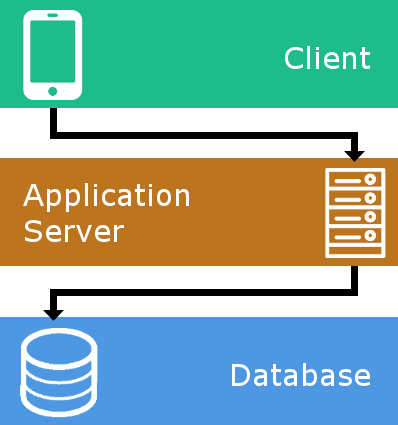
\includegraphics[scale=0.8]{images/highlevelstructure}
\caption{High Level Structure}
\label{ref:highlevelstructure}
\end{figure}

\clearpage
\subsection{Component View}
\subsubsection{High-Level Component View}
\begin{figure}[!h]
\centering
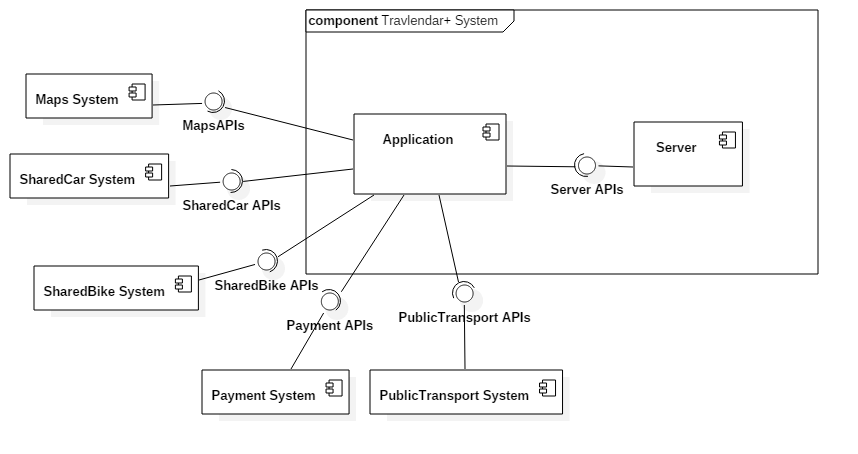
\includegraphics[scale=0.4]{images/ComponentDiagramSystem}
\caption{High Level Component View}
\label{ref:highlevelcomponentview}
\end{figure}
Component to be developed:
\begin{itemize}
\item
\textbf{Application:} It is the core of the system, it manages all information provided by the others services and performs the majority of the functions. It provides the client access to the entire system.
\item
\textbf{Server:} This component has a backup role. It receives the data from the application and provides them when necessary (e.g. during the login operation).
\end{itemize}
Component to be integrated in the system:
\begin{itemize}
\item
\textbf{MapsSystem:} It is the provider of the maps and all necessary information for the computation of the journey.
\item
\textbf{SharedCarSystem, SharedBikeSystem:} Those component provide all information (availability, location and costs) respectively shared cars and shared bikes.
\item
\textbf{PublicTransportSystem:} It provides all information about the public transport of the city.
\item
\textbf{WeatherSystem:} It provides the weather forecasts in the city.
\item
\textbf{PaymentSystem:} This component provides the payment service.
\end{itemize}

\clearpage
\subsubsection{Application System}
\begin{figure}[!h]
\centering
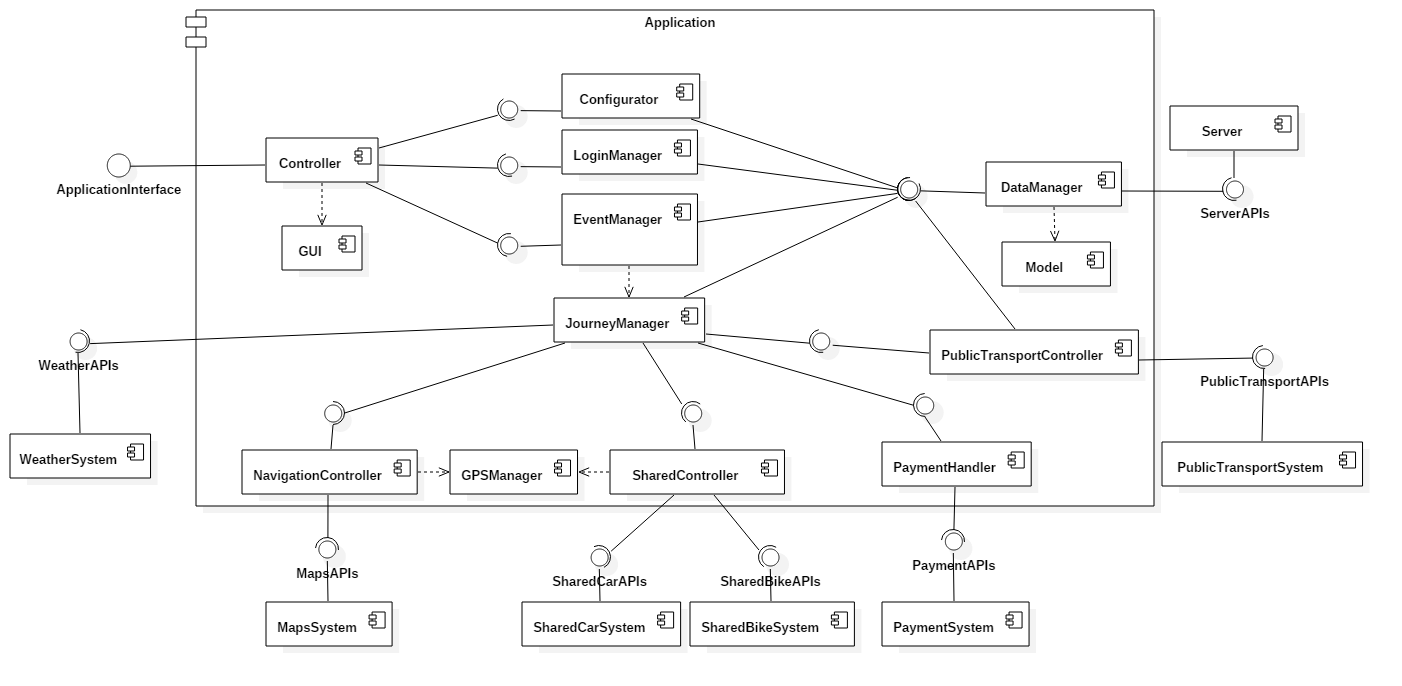
\includegraphics[scale=0.35]{images/ComponentDiagramApplicationSystem}
\caption{Application Component Diagram}
\label{ref:componentdiagramapplicationsystem}
\end{figure}
\begin{itemize}
\item
\textbf{NavigationController:} The component that provides navigation utilities using the Maps APIs and GPS.
\item
\textbf{GPSManager:} The component that handles and gives the GPS information.
\item
\textbf{SharedController:} The component that provides information of all shared systems.
\item
\textbf{PaymentHandler:} The component that handles the payment operations to buy a ticket for a public transport. It ensures that the user is able to successfully complete the payment.
PublicTransportController: The component manages the availability information and the timetable of all public transport.
\item
\textbf{DataManager:} The component that implements and provides through an appropriate interface the methods for accessing the data of our system and it takes care to send the data to the server.. This intermediate component between the entities of the the model and the other components will facilitate extendibility.
\item
\textbf{Model:} It represent how the data are structured (specified in distinct diagram) in the application and ready to be stored by the server on the database.
\item
\textbf{LoginManager:} The component that handles the login operation.
\item
\textbf{Configurator:} The component that offers the configuration functionalities
to customize a set of parameters of the user account.
\item
\textbf{Event Manager:} The component that handles the operations to create and manage an event.
\item
\textbf{Journey Manager:} It manages the user journey.
\item
\textbf{View Controller:} The component that handles the update of the GUI and the retrieval of the user input through the interface.
\item
\textbf{GUI:} Implementation of the presentation layer of the application.
\end{itemize}

\subsubsection{Server System}
\begin{figure}[!h]
\centering
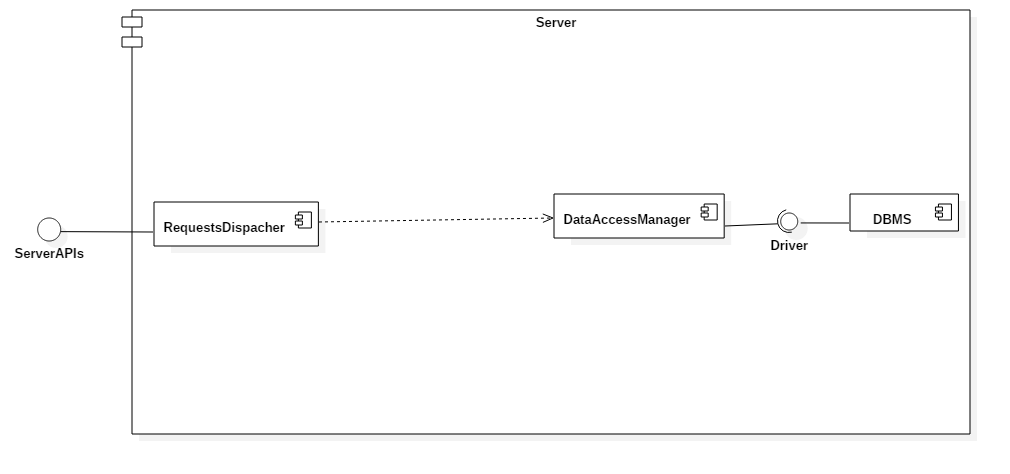
\includegraphics[scale=0.4]{images/ComponentDiagramServer}
\caption{Server Component Diagram}
\label{ref:componentdiagramserver}
\end{figure}
\begin{itemize}
\item
\textbf{RequestDispatcher:} It handles the requests from the application.
\item
\textbf{DataAccessManager:} The component that manages access to the database using a specific driver.
\item
\textbf{DBMS:} The system that will take care of the management of the data, integrated in our system using a specific driver.
\end{itemize}


\clearpage
\subsection{Deployment View}
This diagram purpose is to show the hardware components of our system and where the code is going to run.
\begin{figure}[!h]
\centering
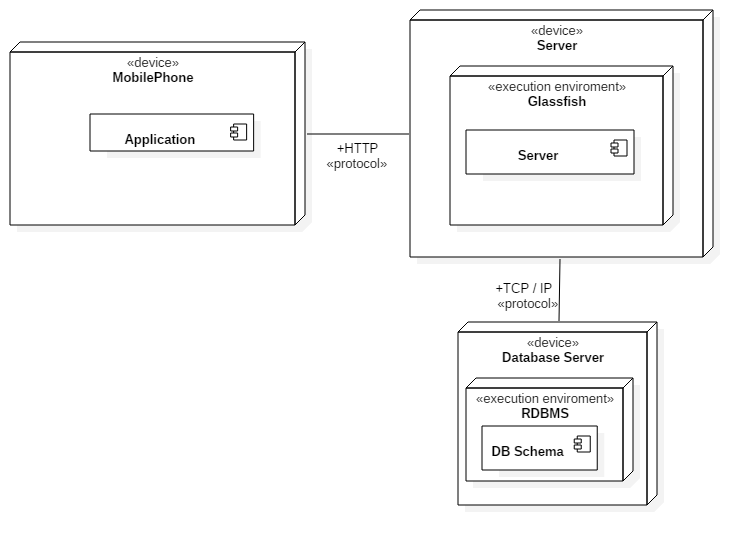
\includegraphics[scale=0.4]{images/DeploymentDiagram}
\caption{Deployment Diagram}
\label{ref:deploymentdiagram}
\end{figure}

\clearpage
\subsection{Runtime View}

\subsubsection{Visitor Registration}
\begin{figure}[H]
\centering
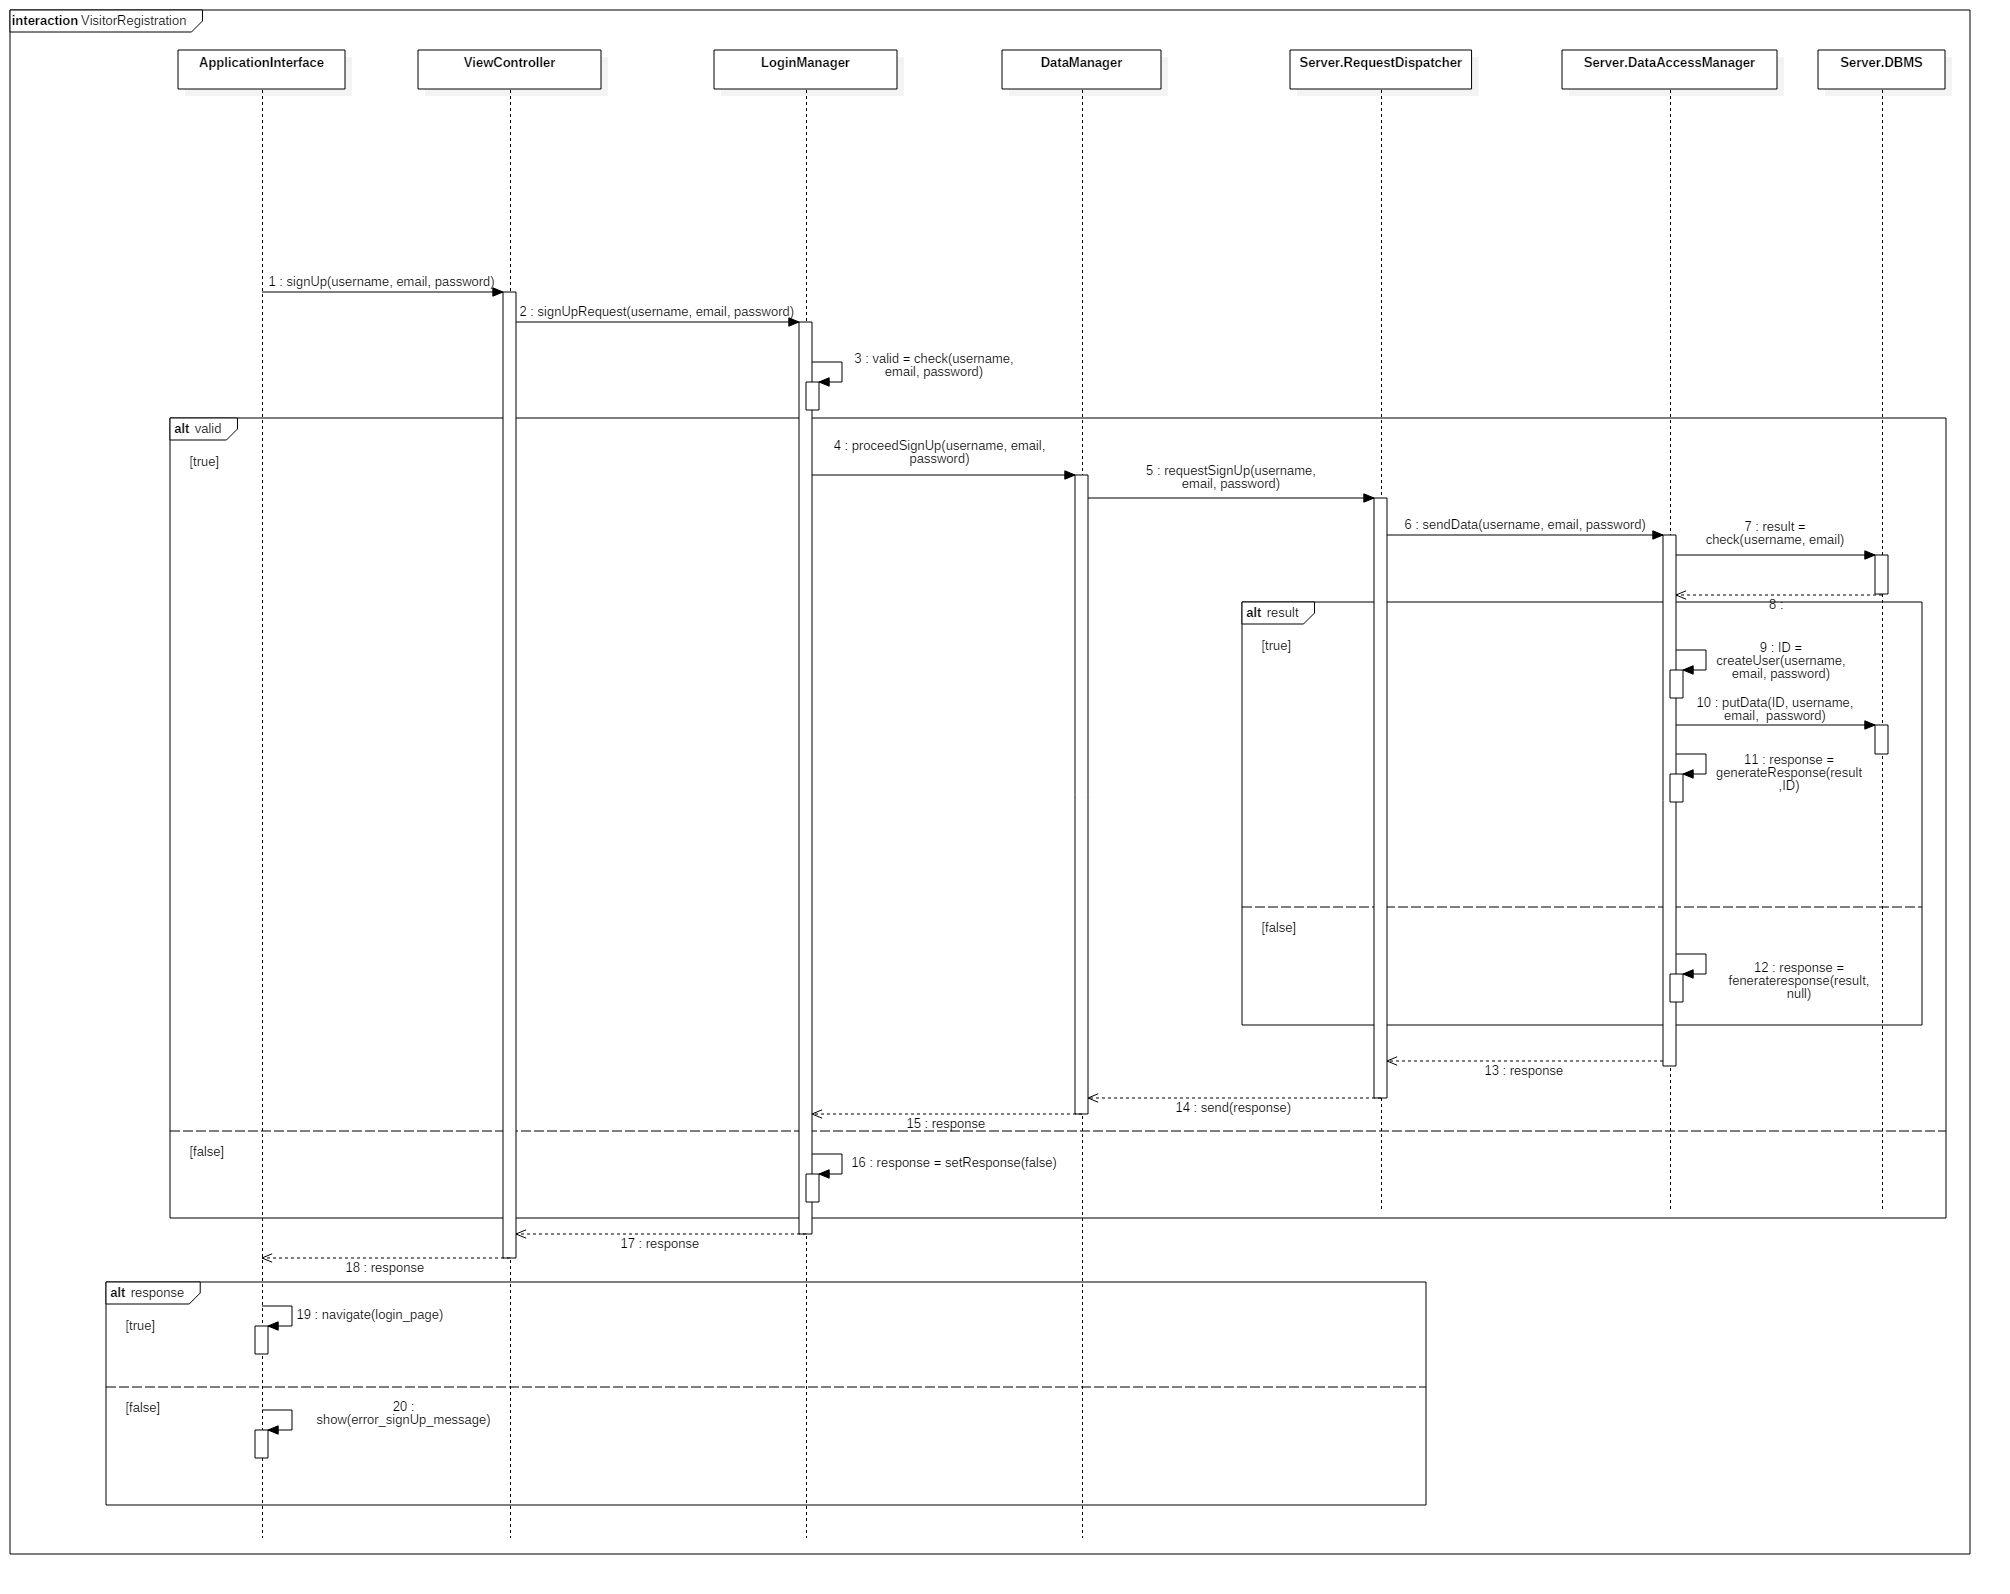
\includegraphics[scale=0.25]{images/VisitorRegistration}
\caption{Visitor Registration}
\end{figure}In this runtime diagram you can see the registration process on the application. The informations are sent by the ApplicationInterface to the Controller that forwards them to the specific manager, in this case the LoginManager. The LoginManager checks if the username and the email are typed correctly or not, if not it returns a negative response. Otherwise the LoginManager proceeds with sign up process by sending the data to the DataManager which calls the server. The server manages the requests with the RequestDispatcher and sends the data to the DataAccessManager that calls the DBMS to check the availability of the username and password. If they are available, the DataAccessManager creates an ID and associates it to the user. The system returns a response the the ApplicationInterface that shows a confirmation or error dialog respectively in case of positive or negative response.

\subsubsection{User Login}
\begin{figure}[H]
\centering
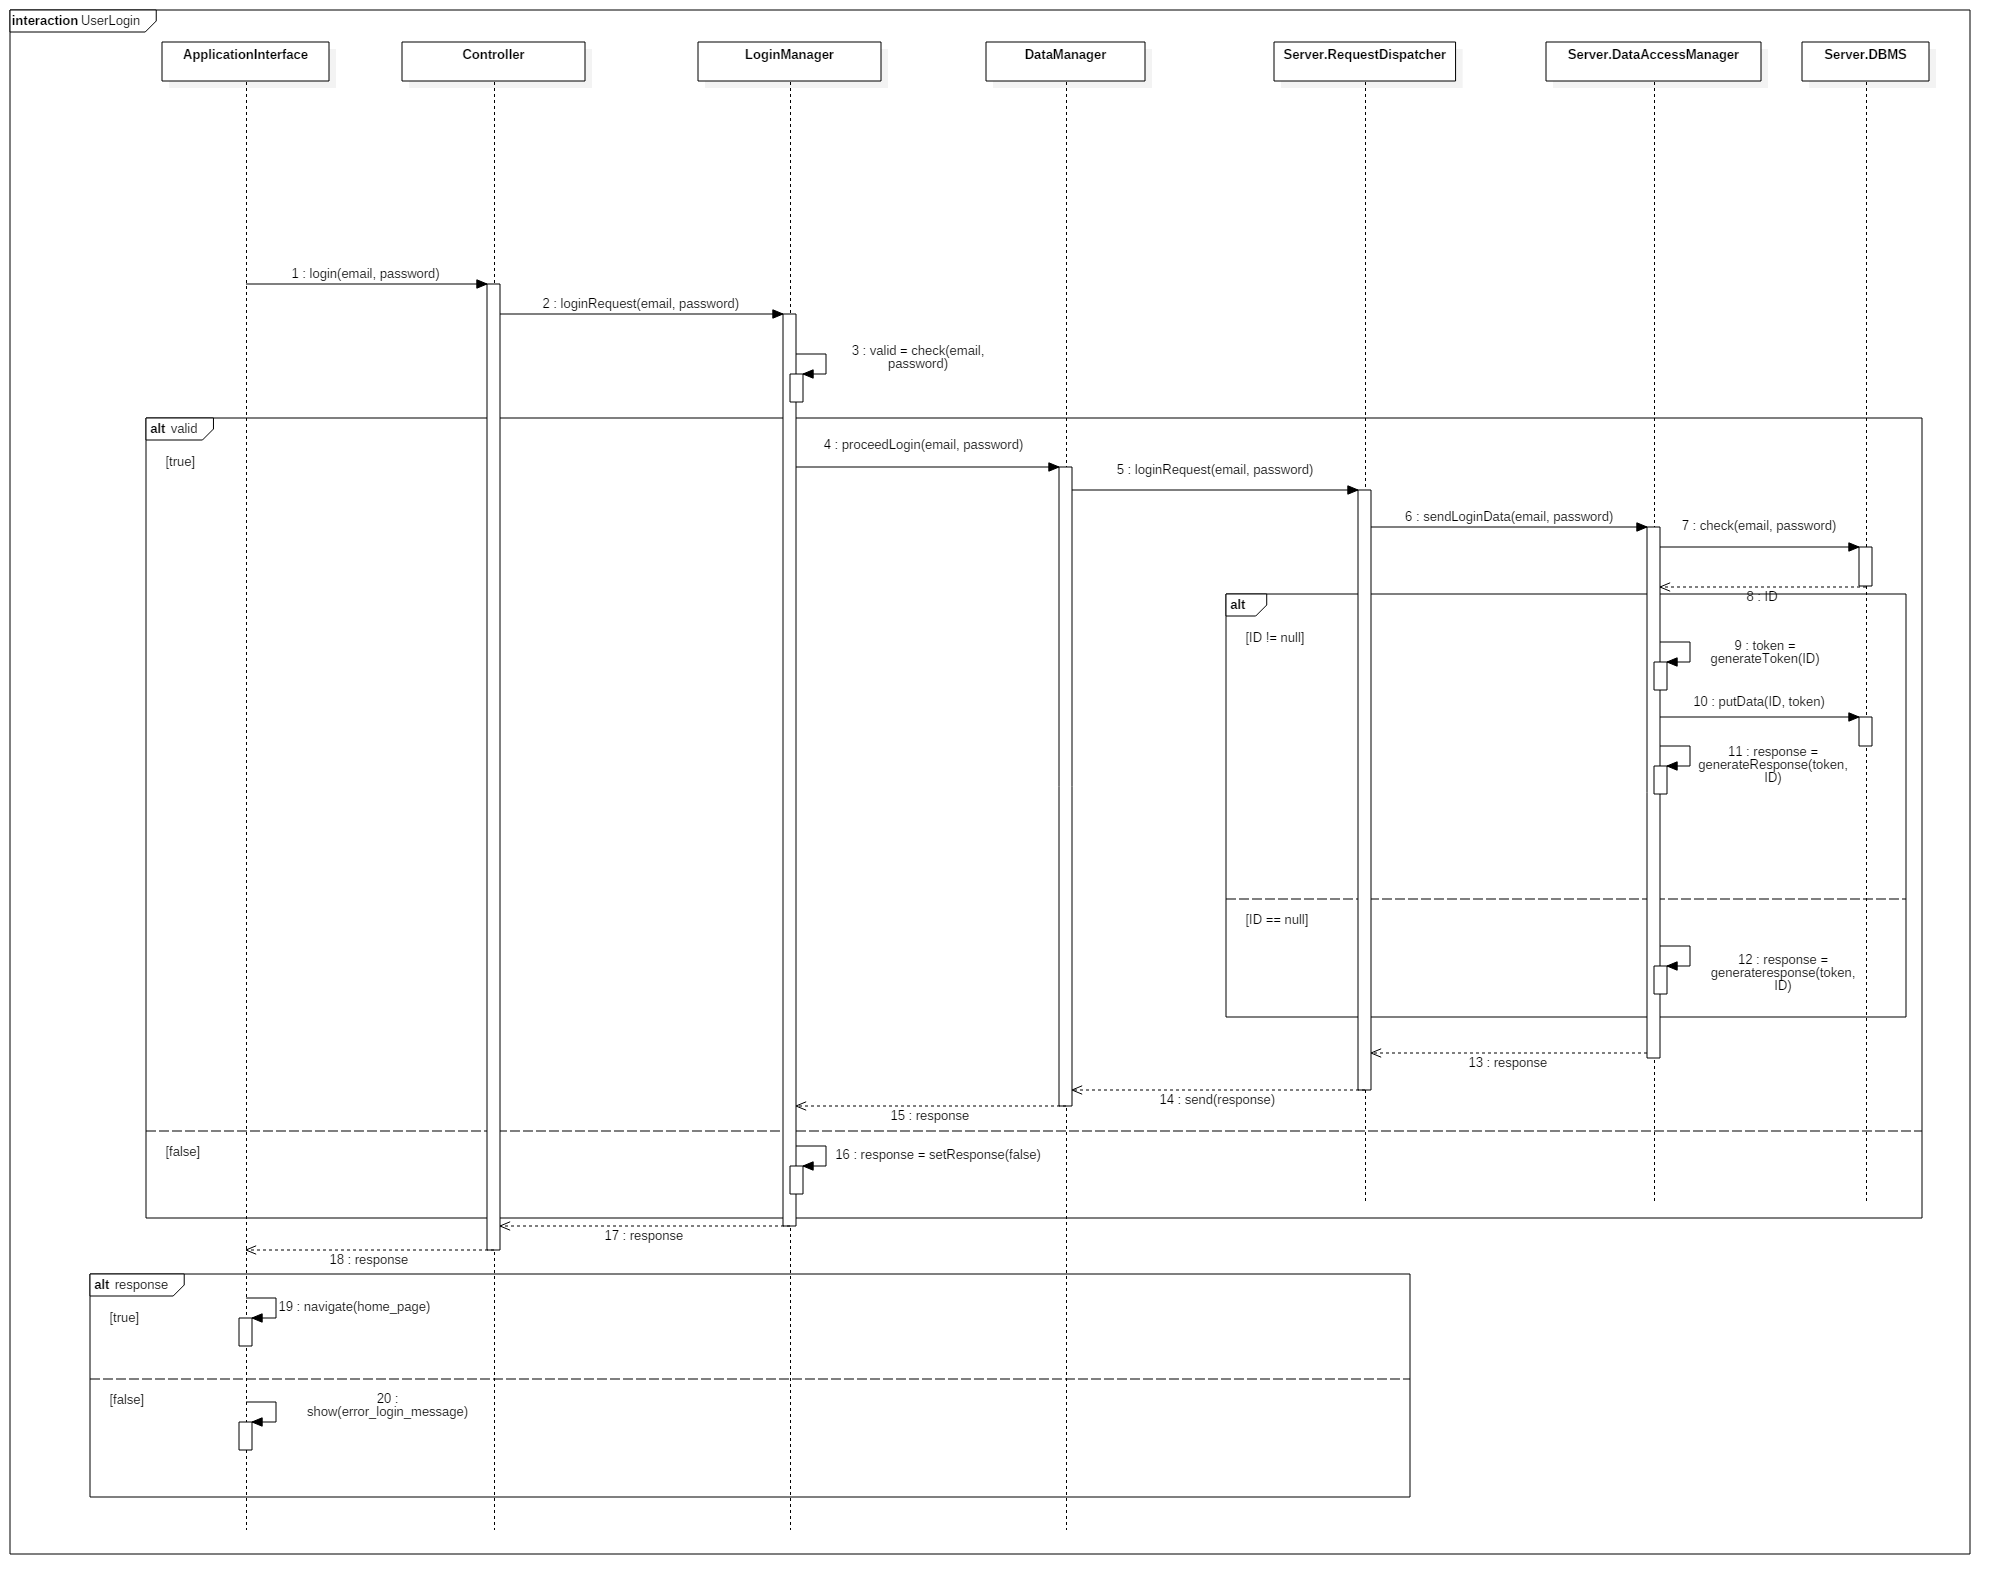
\includegraphics[scale=0.25]{images/UserLogin}
\caption{User Login}
\end{figure}In this runtime diagram you can see the login process for a user that is already registered in the application. The login information are sent by the ApplicationInterface to the Controller that calls the LoginManager. The LoginManager checks if the parameters are typed correctly. If the parameters are not valid the LoginManager generates a negative response, if it is valid he proceeds with the login process and passes the data to the DataManager that makes a request to the server. The RequestDispatcher on the server manages the requests and queries the DBMS through the DataAccessManager to check the data. If data are already present in the DBMS, the DataAccessManager generates a token and stores it in the DBMS, then it generates a positive response; if data are not present the DataAccessManager generates a negative response. In case of positive or negative response the ApplicationInterface redirects the user to the home page or to an error message.

\subsubsection{Setup Preferences}
\begin{figure}[H]
\centering
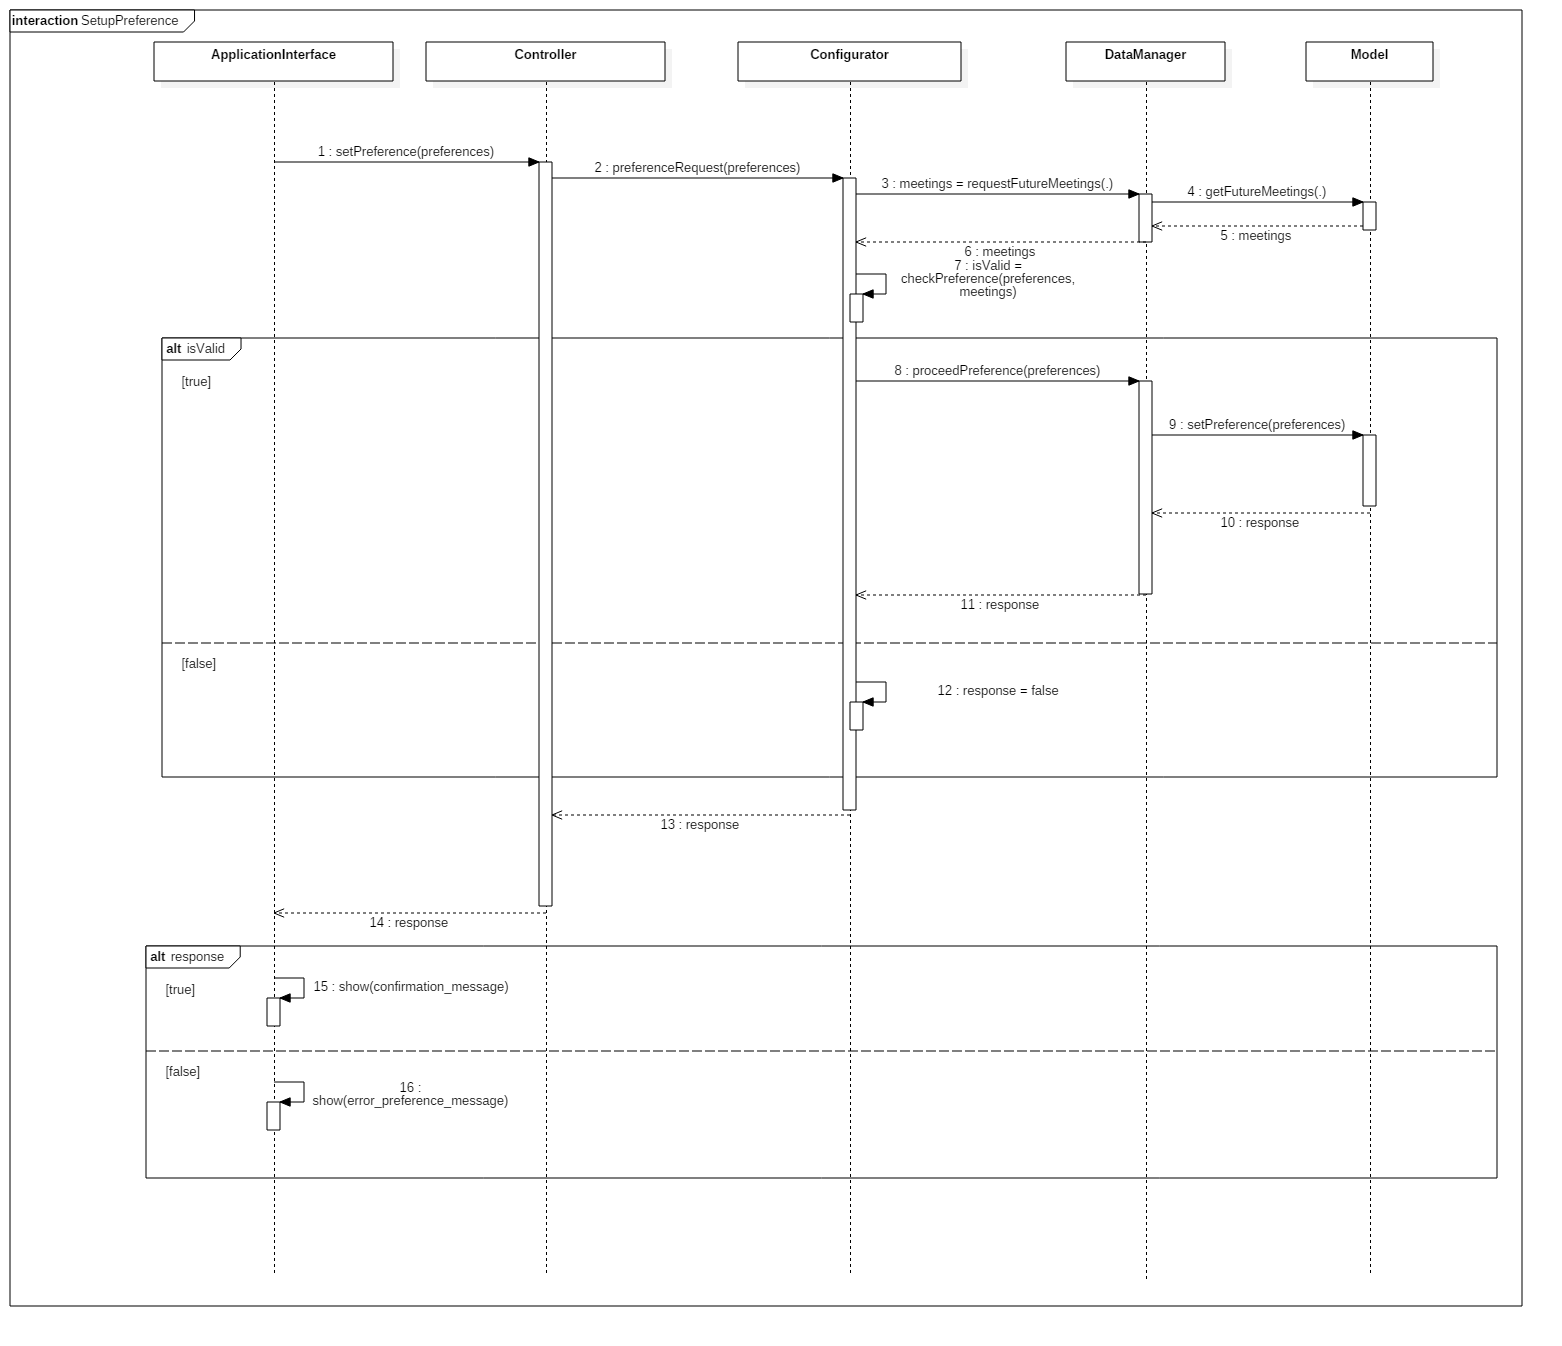
\includegraphics[scale=0.25]{images/SetupPreference}
\caption{Setup Preferences}
\end{figure}This diagram shows how the user can set his preferences. The ApplicationInterface sends all the preferences set by the user to the Controller, which makes a request to the Configurator. The Configurator is the component that manages the preferences, it requests to the DataManager the future meetings that are already present in the Model and checks the correctness of the data. If the preferences are valid, they are passed to the DataManager that puts them in the Model; if the data are not valid it generates a negative response. Depending on the answer, the ApplicationInterface shows a confirmation or error message.

\subsubsection{Create Meeting}
\begin{figure}[H]
\centering
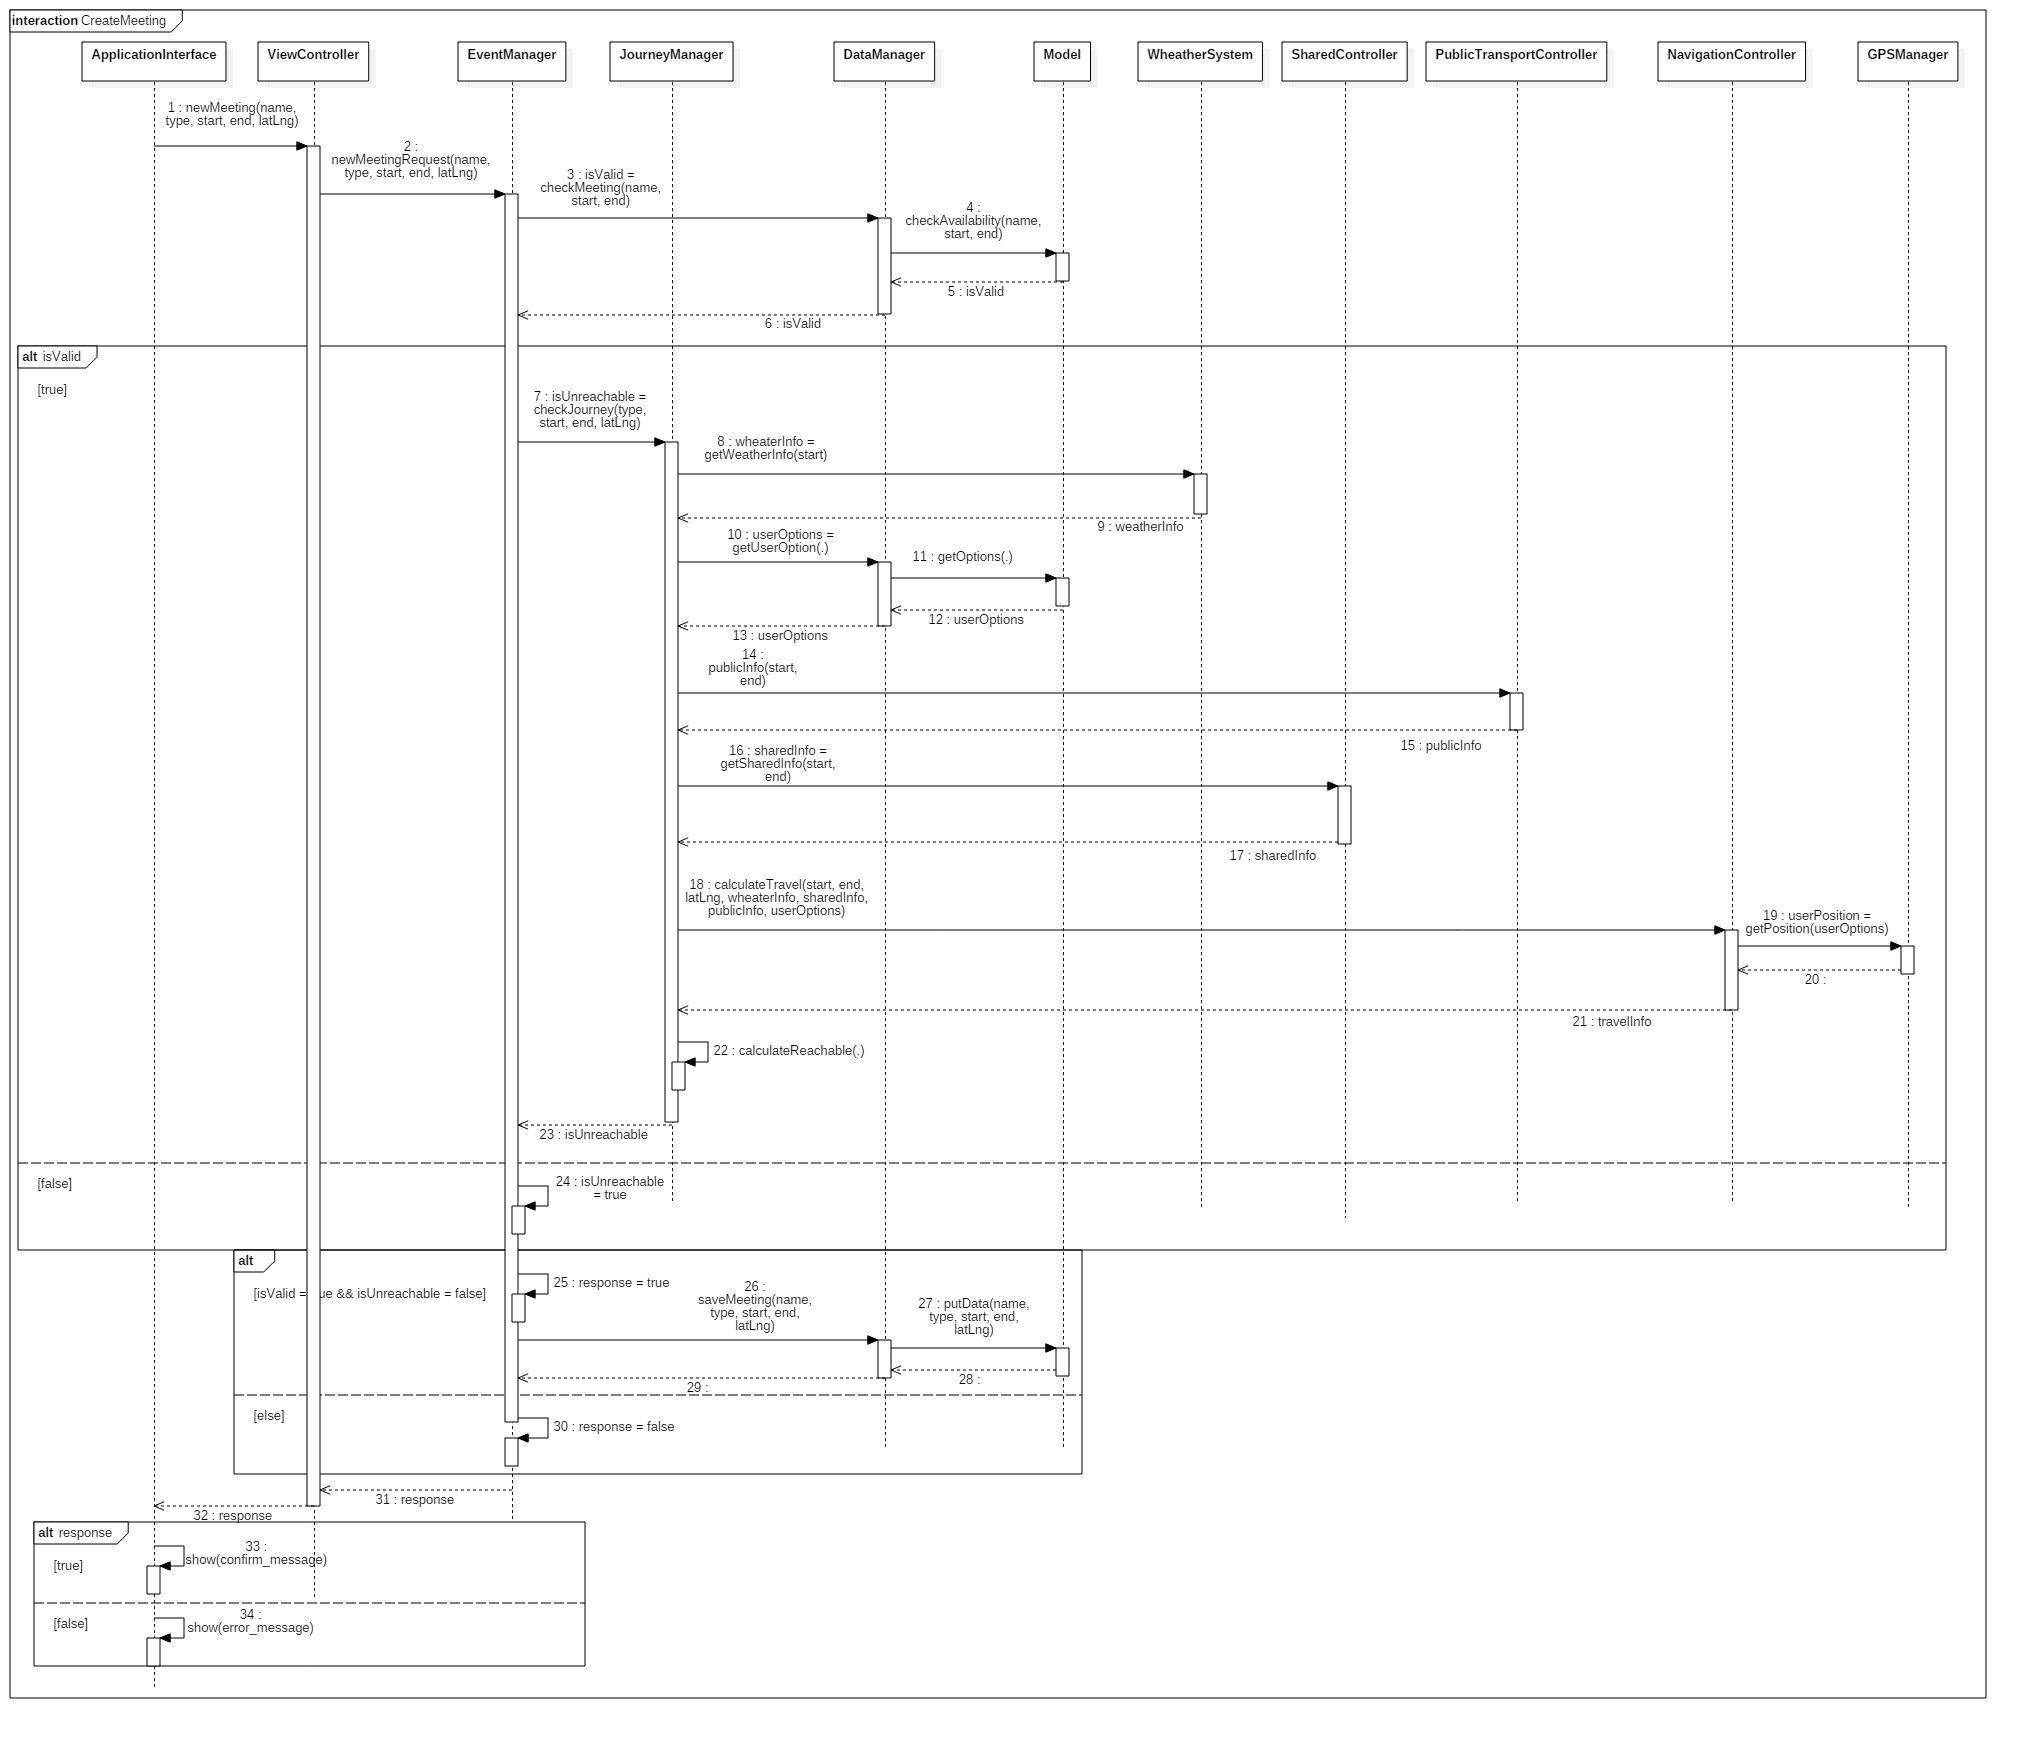
\includegraphics[scale=0.25]{images/CreateMeeting}
\caption{Create Meeting}
\end{figure}This diagram shows the process to create a new meeting. The ApplicationInterface retrieves all information about the meeting that the user wants to create and sends them to the ViewController that calls the EventManager component.The EventManager requests all the meetings of the day of the new one to the DataManager and checks if there is an overlap with other events. If this is the case the event can’t be created and an error message is shown. Otherwise the event is valid and the EventManager takes the information of the previous and the next events and creates an object meeting for the new event. To find the best journey the JourneyManager calls different components to retrieve the information that it needs: the WheaterController for weather information, the DataManager and the Model for the user’s preferences and the NavigationController, which calls the PublicTransportController for the information about hours and availability of public transportations and then calculates all the possible journeys. After that the JourneyManager computes the best journey within all the available ones, taking in consideration the user’s preferences and the weather information.
Eventually, a control is performed to check if the events would be reachable and if the travels leave enough time for lunch.
Finally if all the controls succeed the EventManager saves the meeting into the Model, updates the relative journeys, the lunch time and returns a response to the ApplicationInterface that shows a confirmation or error message.

\subsubsection{Travel to the Meeting}
\begin{figure}[H]
\centering
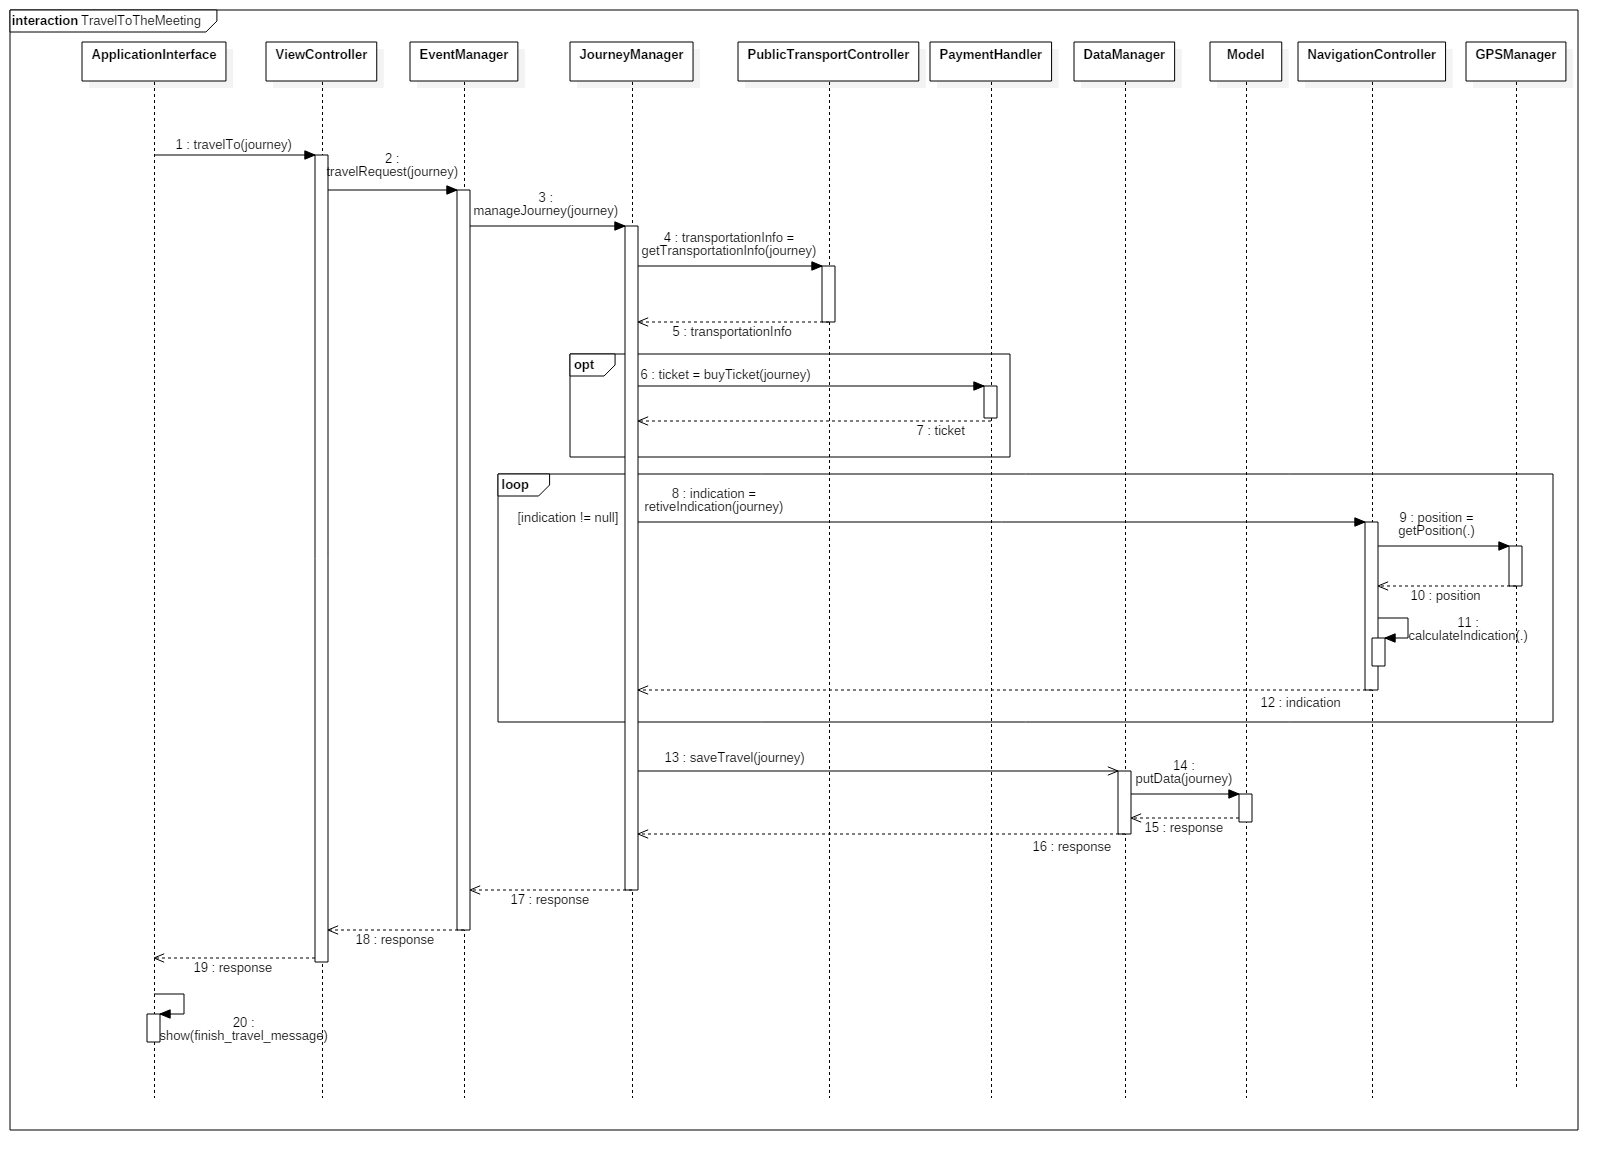
\includegraphics[scale=0.25]{images/TravelToTheMeeting}
\caption{Travel to the Meeting}
\end{figure}This diagram shows the flow of method calls and events that are performed when the user is traveling to a meeting.
The user starts the navigation in the ApplicationInterface which, through the ViewController and the EventManager, passes the relative journey to the JourneyManager.
For each segment that composes the journey, the JourneyManager reads the travel mean, and in case it is a public transport mean, it requests to the DataManager if there is a relative ticket. If there isn’t, the user can opt to buy one.
In case a new ticket is bought, the application saves it and its information in the model. Then, when the users starts the navigation the NavigationController begins showing directions.
Every time the user position changes, the GPS Manager sends an asynchronous call to the Navigation Controller.  From the new position, the NavigationController calculates the directions and sends them to the ApplicationInterface which shows them to the user. The navigation ends when the user location is equal to the final destination of the segment.
When the navigation ended and the user arrives at the meeting location, the JourneyManager updates the journey information in the Model and saves it as completed; then it send a response to the ApplicationInterface that shows a confirmation or error message to the user.


\clearpage
\subsection{Component Interfaces}
The server communicates with the DBMS via the JPA over standard network protocols. Thus, the DB and the server layers can be deployed on different tiers, as well on the same one.\\
The low-level technicalities about the specific dialect of SQL for the selected DBMS are abstracted by the JPA, which also deals with the O/R mapping.\\
The mobile app shall communicate with the server using the back-end programmatic interface presented in the component view and implemented as a RESTful interface over the HTTPS protocol. The RESTful interface is implemented in the application server using JAX-RS and uses JSON as the data representation language.
\\
\begin{figure}[H]
\centering
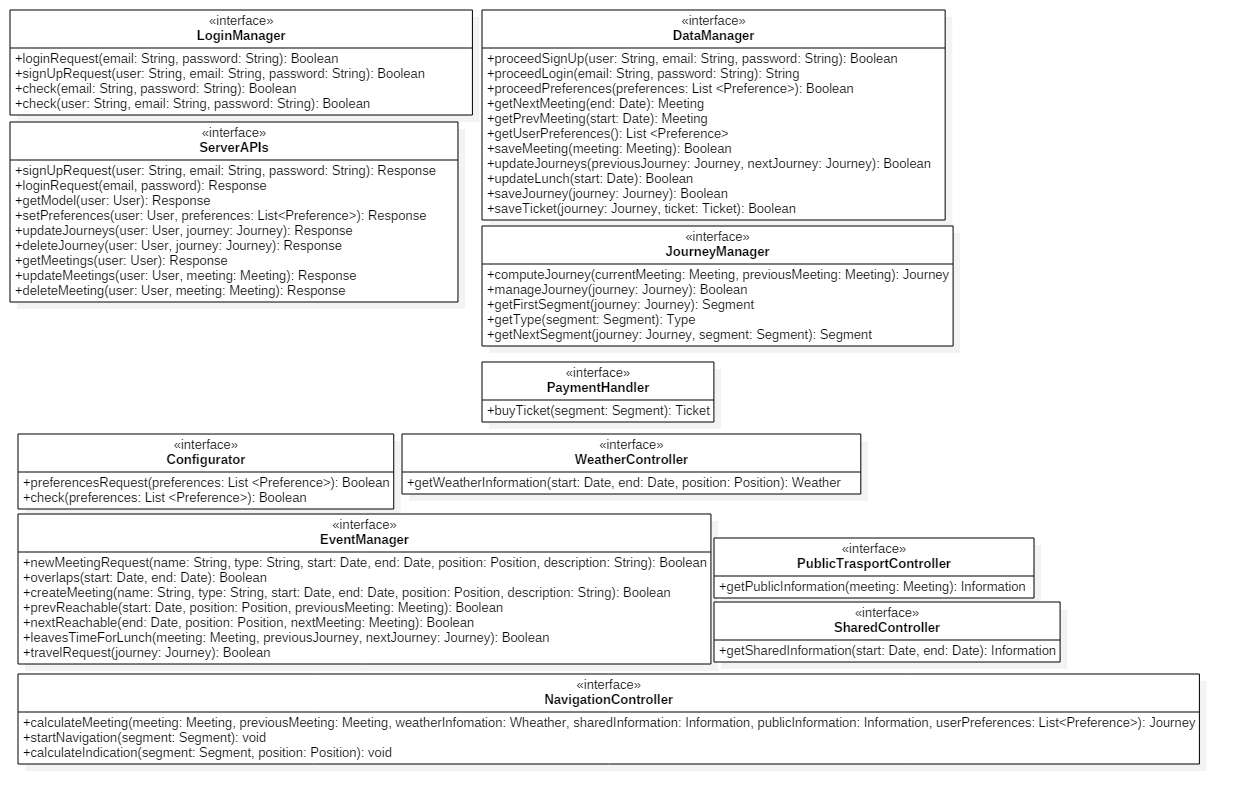
\includegraphics[scale=0.4]{images/componentInterfaces}
\caption{Component Interfaces}
\end{figure}
This diagram shows the most relevant parts of the interfaces that our system is going to use for communication between the various components.

\clearpage
\subsection{Selected Architectural styles and patterns}
The following architectural styles and patterns have been used:
\begin{itemize}
\item
\textbf{Observer pattern:} This pattern is used between NavigationController and Controller. It allows the NavigationController to update the user’s view with new directions in a transparent way when the position changes.
\item
\textbf{Model-Control-View:} It is used for the main components of the system. It’s a really good choice of design that allows to keep clear the role of every component and that makes the system easier to deploy and maintain.
\item
\textbf{Client-Server:} This pattern is a good practice for a distributed system. It is used between the application server (client) queries the DB (server) and the application (client) communicates with the application server.
\item
\textbf{Service-oriented Architecture:} It is used by the system for the communication between the server and the user’s device (RESTful). The SOA allows to think at a higher level of abstraction, by looking at the component interfaces and not at their specific implementation. SOA style also improves modularity: by making service description, discovery and binding explicit, it is easier to build new plugins and test single modules independently.
\item
\textbf{Fat Client:} The fat client paradigm is implemented because the interaction between user’s device and the server hasn’t a central role in the system behavior . Having a fat client in our case is an advantage because most application logic is on the user’s device, which has sufficient computing power and is able to manage concurrency issue efficiently.
\end{itemize}